\section{Software Requirement Analysis}
Software requirement analysis is a process of gathering and interpreting facts, diagnosing problems and the information to recommend improvements on the system. It is a problem solving activity that requires intensive communication between the system users and system developers. System analysis or study is an important phase of any system development process. System analysis is concerned with becoming aware of the problem, identifying the relevant and decisional variables, analyzing and synthesizing the various factors and determining an optimal or at least a satisfactory solution or program of action.\\

\noindent A detailed study of the process must be made by various techniques like interviews, questionnaires etc. The data collected by these sources must be scrutinized to arrive to a conclusion. The conclusion is an understanding of how the system functions. The proposal is then weighed with the existing system analytically and the best one is selected. The proposal is presented to the user for an endorsement by the user. The proposal is reviewed on user request and suitable changes are made. This is loop that ends as soon as the user is satisfied with proposal.\\

\subsection{Functional Requirements}
\begin{itemize}
\item {\bf Specific Requirements}: This phase covers the whole requirements 
for the system. After understanding the system we need the input data 
to the system then we watch the output and determine whether the output 
from the system is according to our requirements or not. So what we have 
to input and then what we'll get as output is given in this phase. This 
phase also describe the software and non-function requirements of the 
system.
\item {\bf Input Requirements of the System}
\begin{enumerate} 
\item Guess points
\item Precision
\item User can define his/her requirement.
\end{enumerate}
\vskip 0.5cm
\item {\bf Output Requirements of the System}
\begin{enumerate} 
\item Final output in form of Certificates. 
\item Taking bulk input values in form of Csv.
\end{enumerate}
\vskip 0.5cm
\item {\bf Software Requirements}
\begin{enumerate} 
\item Language: Libre-Office
\item Web Languages: php
\item Documentation: \LaTeX{}
\item Operating System: Any

\end{enumerate}
\vskip 0.5cm
\subsection{Non functional requirements}
\begin{enumerate} 
\item Scalability: System should be able to handle a number of users. 
For e.g., handling around thousand users at the same time.
\item Usability: Simple user interfaces that a layman can understand.
\item Speed: Processing input should be done in reasonable time
 i.e. we can say maximum 24 hrs.
\end{enumerate}

\item{\bf Users of the System}
\begin{enumerate} 
\item Client : Clients are the end users that benefit from this software.
They just provide input and gets output.Client of this system:
\begin{enumerate}
\item Researcher or student
\end{enumerate}
\end{enumerate}
\end{itemize}
\section{Flowchart}
A flowchart is a type of diagram that represents an algorithm, work flow or process, showing the steps as boxes of various kinds, and their order by connecting them with arrows. 
Flowcharts are used in designing and documenting simple processes or programs. Like other types of diagrams, they help visualize what is going on and thereby help understand a process, and perhaps also find flaws, bottlenecks, and other less-obvious features within it. There are many different types of flowcharts, and each type has its own repertoire of boxes and notational conventions. The two most common types of boxes in a flowchart are:
\begin{enumerate}
\item A processing step, usually called activity, and denoted as a rectangular box.
\item A decision, usually denoted as a diamond.
\end{enumerate}
Following is flowchart of system showing flow of control and Data in the software-:
\begin{figure}[!ht]
\centering
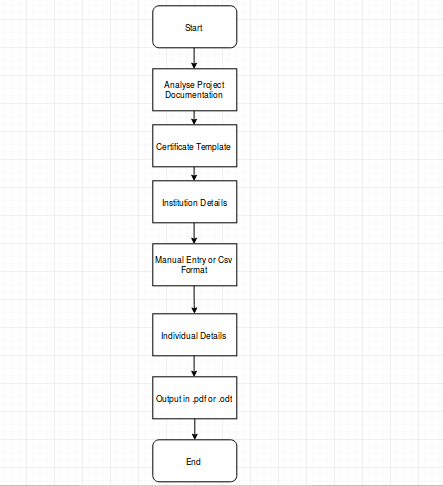
\includegraphics[width=1\textwidth]{images/design.png}                   
\caption{Flowchart of project}
\hspace{-1.5em}
\end{figure}

